\section{Absolute Performance and Operating Conditions}\label{sec:performance}
\subsection{Completion and performance magnitudes}
All 5,760 cells complete all 200 requests. There is no administrative-horizon
censoring and no missing cell-level ranking endpoint. The 1,152,000 request
executions are repeated conditions on the 24,000 underlying records, not
independent observations. Individual TPOT excludes one-output-token
requests, leaving 103--200 observations per cell. Cell mean latency ranges
from 0.008314 to 3.893923 simulated seconds, p95 latency from 0.008560 to
7.300052 seconds, and output-token throughput from 332.489 to 7,766.685
tokens per simulated second. These magnitudes describe the fixed-cost model.

Figure~\ref{fig:absolute} shows every source/setting/capacity combination,
with equal-window means. Appendix Table~\ref{tab:absolute} gives compact
source/capacity aggregates. The SLO-gated adaptation reduces aggregate
mean latency relative to chunked-FCFS in all six source/capacity groups,
by 11.3--34.0\%. Yet token throughput falls by 1.65--4.01\% in those same
groups. On BurstGPT, mean window-p95 latency increases by 3.72\% with
four residents and 18.97\% with eight, despite better mean latency and
ANWG. On Bailian with four residents, ANWG decreases by 3.12\% despite
24.05\% lower mean latency. Lower average response time therefore does
not imply better tails, completion-by-deadline utility or throughput.

\begin{figure}[!htbp]
\centering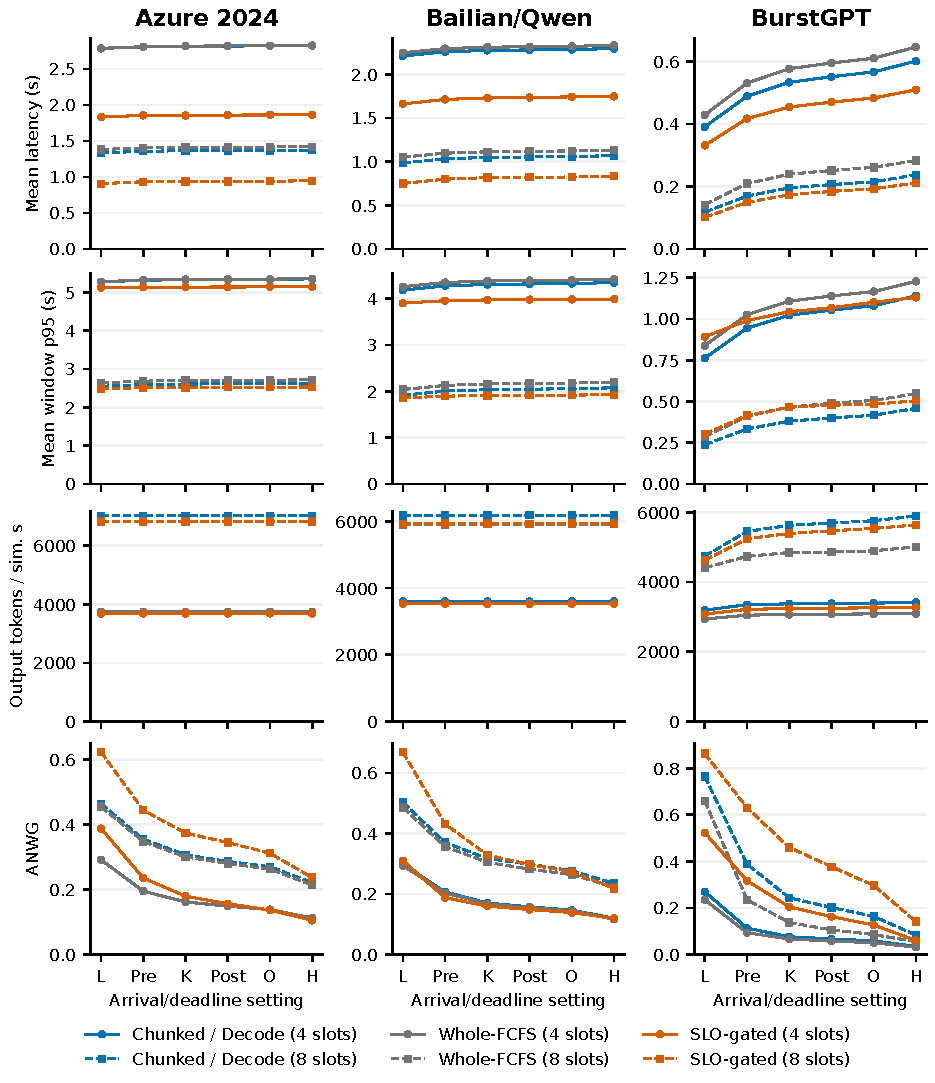
\includegraphics[width=\linewidth]{figures/absolute.pdf}
\caption{Absolute performance: 40 equally weighted windows per point.
L/Pre/K/Post/O/H denote the six inherited settings, not measured CM-0.1
saturation regimes. Solid/dashed lines allow four/eight reserved residents.
Chunked-FCFS and decode-first coincide exactly. Seconds and throughput
refer to simulated time; p95 panels average window-level p95s. No sampling
confidence intervals are implied.}\label{fig:absolute}
\Description{Twelve panels show mean latency, mean window p95 latency,
token throughput and ANWG by inherited setting for Azure, Bailian and
BurstGPT. SLO-gated has lower aggregate mean latency but lower throughput;
its BurstGPT tail latency is worse at both capacities.}
\end{figure}

\subsection{Matched-window trade-offs}
Figure~\ref{fig:matched} retains all 40 windows per source and both
capacities. Each point averages six \emph{matched differences} within a
window; it does not pool requests or substitute a difference between
unmatched supports. The combination of lower mean latency and worse tail
latency is visible on BurstGPT, while the size of the mean improvement
varies appreciably by window and capacity. Throughput losses accompany
many mean-latency improvements. Complete per-condition differences remain
in the frozen analysis, and the plotted window summaries are supplied as
CSV data.

SLO-gated is the unique mean-latency winner in 1,146 of 1,440 conditions,
but the unique p95-latency winner in only 834 and the unique token-throughput
winner in 482. Its unique ANWG wins number 1,004. The mean-latency count
splits into 480/480 Azure, 468/480 Bailian and 198/480 BurstGPT conditions.
These counts describe exact optima, not their practical margins. They
complement the absolute differences rather than override the unfavorable
throughput and tail outcomes.

\begin{figure}[!htbp]
\centering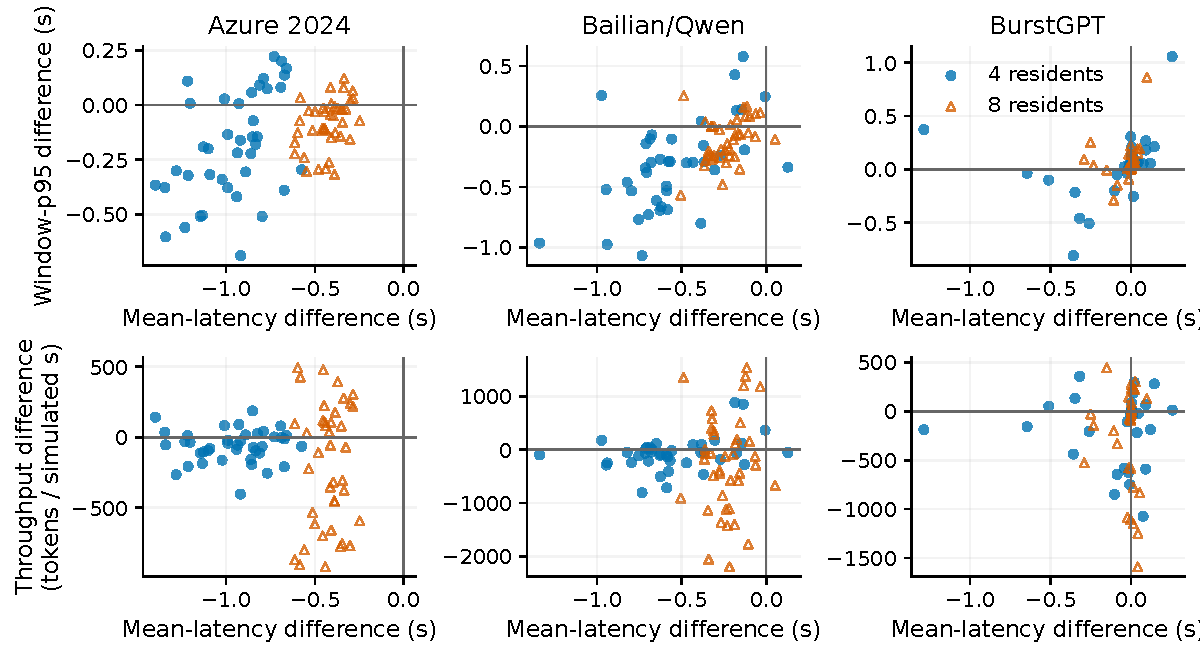
\includegraphics[width=\linewidth]{figures/matched.pdf}
\caption{SLO-gated minus chunked-FCFS for every window, averaged over its
six matched settings. Each panel has 40 windows at each of two capacities.
Leftward means lower mean latency; upward means worse window-p95 latency
(top) or higher throughput (bottom). These are descriptive points with no
independent-sampling interpretation.}\label{fig:matched}
\Description{Six scatter panels compare matched mean-latency differences
against p95 and throughput differences by source. Both capacity groups
and negative outcomes are retained.}
\end{figure}

\subsection{Reservation and setting sensitivity}
Doubling KV reservation capacity permits eight rather than four residents.
At the source/capacity aggregate level, this improves throughput and lowers
mean and mean-window-p95 latency for every adaptation. Actual used KV peaks
at 47,872 tokens in the smaller-capacity runs and 62,880 in the larger ones,
both below even the smaller nominal capacity. The observed constraint is
full-context reservation-induced concurrency, not exhaustion of used KV
at the nominal token limit. Paging, eviction and native memory-pressure
benefits cannot be inferred from this comparison.

Inherited settings can change goodput substantially while leaving aggregate
throughput almost unchanged. For Azure chunked-FCFS with four residents,
LOW to HIGH\_PRESSURE changes mean latency from 2.7858 to 2.8269 seconds
and token throughput from 3,745.9 to 3,746.3, while ANWG falls from
0.291375 to 0.112625. Equation~\ref{eq:scaling} explains why interpreting
this as an arrival-rate effect alone would be incorrect: the deadline
criterion becomes tighter at the same time.

\paragraph{Answer to RQ1.}
Under this reservation-limited contract, the complete corpus exhibits a
mean-latency/throughput trade-off with source-specific tail and goodput
costs. Capacity changes the permitted concurrency; inherited settings
jointly change arrivals and deadline slack. Completion is universal here,
so the reported trade-offs do not result from selectively omitting
unfinished requests. Their magnitudes are informative even where ranks
remain unchanged.

\FloatBarrier
